\chapter{Results and Evaluation}
In this chapter we are going to show the best results obtained by setting up the training phase as described in the previous chapters. Most of the parameter tuning was done on just one dataset\footnote{The Reuters Corpus, RCV1}, and then the same setup was used to produce results for all our datasets.

\section{Confusion matrix}
A confusion matrix is a table that is often used to describe the performance of a classification model (or \enquote{classifier}) on a set of test data for which the true values are known.
To help the reader better understand what this is all about, we can give a practical example with authorship attribution. Suppose we have an unknown document and we have a verification problem where we have to indicate whether Shakespeare is the author of the unknown document or not.
The confusion matrix takes the form it has in \autoref{fig:confusion_matrix} and 4 types of values show up:

\begin{itemize}
	\item \textbf{true positives (TP)}: These are cases in which we predicted yes (Shakespeare is the author of the unknown document), and he really was the author of that document.
	\item \textbf{true negatives (TN)}: We predicted no, and he didn't write that document.
	\item \textbf{false positives (FP)}: We predicted yes, but he didn't actually write that document. (Also known as a "Type I error.")
	\item \textbf{false negatives (FN)}: We predicted no, but in reality he did write that document. (Also known as a "Type II error.")
\end{itemize}

These aforementioned definitions will come in very handy to better understand all the metrics used to evaluate the model we built.

\begin{figure}[ht]
	\centering
	\includegraphics[width=.8\textwidth, height=0.8\textheight, keepaspectratio]{confusion_matrix}
	\caption[Confusion matrix example]{A confusion matrix example with 4 classes of values: true positive, true negative, false positive and false negative.}
	\label{fig:confusion_matrix}
\end{figure}

\section{Metrics used}
In order to evaluate the performance of the model being built, we computed for each training phase, 2 different scores on the testing set: the \textit{accuracy score} and the \textit{F1 score}\footnote{\url{http://scikit-learn.org/stable/modules/generated/sklearn.metrics.f1_score.html}}.\\ 
The accuracy score, one of the more obvious metrics, is the measure of all the correctly identified authors of each documents. It's mostly used when all the classes are equally important.
\begin{equation}
Accuracy = \frac{True Positive + True Negative}{(True Positive + False Positive + True Negative + False Negative)}
\end{equation}
The F1 score can be interpreted as a weighted average of the precision\footnote{The measure of the correctly identified positive cases from all the predicted positive cases.} and recall\footnote{The measure of the correctly identified positive cases from all the actual positive cases.}, where an F1 score reaches its best value at 1 and worst score at 0. The relative contribution of precision and recall to the F1 score are equal.\\The formula for the F1 score is:\\
\begin{equation}
F1 = \frac{2 * (precision * recall)}{(precision + recall)}
\end{equation}
where:
\begin{itemize}
	\item \textbf{Precision:} is the fraction of relevant instances among the retrieved instances.
	\item \textbf{Recall:} is the fraction of relevant instances that have been retrieved over the total amount of relevant instances.
\end{itemize}

To summarise the differences between the F1 and the accuracy:
\begin{itemize}
	\item Accuracy is used when the True Positives and True negatives are more important while F1 is used when the False Negatives and False Positives are crucial.
	\item Accuracy can be used when the class distribution is similar while F1 is a better metric when there are imbalanced classes.
	\item In most real-life classification problems, imbalanced class distribution exists and thus F1 is a better metric to evaluate our model on.
\end{itemize}

\section{Results obtained over different datasets}

In this section we will present and discuss the best results obtained for the different datasets selected, with particular attention to the type of feature representation, the number of authors, the choice of division between training and testing sets, and whether or not the authors' documents belong to different categories.

\subsection{Reuters Corpus results}

The first results we show refer to the Reuters Corpus as it was the dataset on which we did cross validation and hyperparameters tuning. In fact both the choices of features representation, the parameters and the tokenizer, the classifier parameters were all chosen according to the performance of this corpus, especially in the portion that we called RCV1-50, that is the selection of 100 documents per author, for the 50 most prolific authors of the Reuters corpus, for the CCAT category.\\
Precisely for this reason in \autoref{tab:tableRCV1_50} are shown the 3 best results on this portion of the dataset in terms of both accuracy score and F1. As can be seen from the table, the best results were obtained with the linear SVM classifier, with tfidf as the method of feature representation, and gradually increasing results were obtained thanks to the study of a better selection of words on the tokenizer.
In fact we denote \textit{\enquote{stock\_tokenizer}} the standard tokenizer of the python library 
\textit{sklearn.feature\_extraction.text.TfidfVectorizer}. While in the other two approaches we changed the tokenizer, setting a \enquote{custom} one, at first leaving all words except the text between double quotes. The best result was obtained with a variation of this custom tokenizer, called \textit{\enquote{only-remove-quotes-tokenizer}}, removing the words between double quotes but with a length of greater than one word (i.e. the single words between double quotes were left intact) and in addition we used not only the representation of a word ngram, but we also chose to represent the pair of neighboring words to better identify the author of a text.
The reasoning behind this type of representation and the reason why we got the best result is because the use of words between double quotes could better distinguish the author of a text, while the sentences enclosed by double quotes were discarded because they certainly belong to a quote, and therefore do not distinguish the style of an author.


\begin{table}[h!]
	\begin{center}  
		\caption[Reuters Corpus Results - 50 authors]{Accuracy score and F1 macro score for Reuters Corpus 50 authors CCAT category.} 
		\label{tab:tableRCV1_50}
		%\resizebox{\linewidth}{!}{  %
		\begin{tabular}{| p{5 cm} | c | c |}
			\hline 
			Model & Accuracy & F1\\
			\hline
			LinearSVC (combinedDFs), tfidf, stock tokenizer & 0.7644 & 0.7600 \\ \hline
			LinearSVC (combinedDFs), tfidf, only-remove-quotes-tokenizer & 0.7884 & 0.7842 \\ \hline
			\textbf{LinearSVC (combinedDFs), tfidf, only-remove-quotes-tokenizer (threshold 1),
			ngram=(1,2)} & \textbf{0.7984} & \textbf{0.7949} \\ \hline
			%\bottomrule 
		\end{tabular} 
		%}
	\end{center}
\end{table}

In \autoref{tab:tableRCV1_10} we can see the results of the same models on the portion of the reuters corpus dataset, of the 100 documents extracted by each author, selecting the 10 most prolific authors with the documents belonging to the CCAT category.\\

\begin{table}[h!]
	\begin{center}  
		\caption[Reuters Corpus Results - 10 authors]{Accuracy score and F1 macro score for Reuters Corpus 10 authors CCAT category.} 
		\label{tab:tableRCV1_10}
		%\resizebox{\linewidth}{!}{  %
		\begin{tabular}{| p{5 cm} | c | c |}
			\hline 
			Model & Accuracy & F1 \\
			\hline
			LinearSVC (combinedDFs), tfidf, simple tokenizer & 0.8780 & 0.8760 \\ \hline
			LinearSVC (combinedDFs), tfidf, only-remove-quotes-tokenizer & 0.9080 & 0.9060 \\ \hline
			\textbf{LinearSVC (combinedDFs), tfidf, only-remove-quotes-tokenizer (threshold 1),
			ngram=(1,2)} & \textbf{0.9220} & \textbf{0.9210} \\ \hline
			%\bottomrule 
		\end{tabular} 
		%}
	\end{center}
\end{table}

The Reuters dataset being frequently used in other authorship attribution studies, also allows us to compare the results in terms of accuracy with other models that we are aware of.
In \autoref{tab:tableRCV1_10_benchmark} we can see some of the models that achieved the best results for the authorship attribution task on the Reuters Corpus both for the RCV1-10 portion and for the RCV1-50 portion.
At the end of the table we reported the best result achieved with our method, that for both of the portion of the dataset (i.e. the 10 authors and the 50 authors) showed the highest accuracy score to the best of our knowledge.
\begin{table}[h!]
	\begin{center}  
		\caption[Reuters Corpus Benchmark - 10 and 50 authors]{Accuracy score for Reuters Corpus 10 and 50 authors in the CCAT category.} 
		\label{tab:tableRCV1_10_benchmark}
		%\resizebox{\linewidth}{!}{  %
		\begin{tabular}{| p{5 cm} | c | c |}
			\hline 
			Model & RCV1-10 & RCV1-50 \\
			\hline
			D2V words\cite{posadas2017application} & 0.8280 & 0.7524 \\ \hline
			Local histograms \cite{sari2017continuous} & 0.8640 & - \\ \hline
			Tensor space models \cite{plakias2008tensor} & 0.8080 & - \\ \hline
			Character and word n-grams \cite{sapkota2015not} & 0.7940 & - \\ \hline
			N-gram feature selection \cite{houvardas2006n} & - & 0.7404 \\ \hline
			\textbf{Our approach} & \textbf{0.9220} & \textbf{0.7984} \\ \hline
			%\bottomrule 
		\end{tabular} 
		%}
	\end{center}
\end{table}

For the RCV1-10 portion of the reuters corpus the results of our approach improved the best accuracy score achieved with local histograms method in \cite{sari2017continuous} by $6,71\%$ and for the RCV1-50 we improved by $6,11\%$ the results obtained in \cite{posadas2017application} with the doc2vec words model.


\subsection{GDELT Corpus results}
Regarding the dataset downloaded from the GDELT project, composed of documents belonging to Victorian era books belonging to 45 authors, the 3 best results obtained are shown in \autoref{tab:tableGDELT}. 

\begin{table}[h!]
	\begin{center}  
		\caption[GDELT Results - 45 authors]{Accuracy score and F1 macro score for GDELT 45 authors.} 
		\label{tab:tableGDELT}
		%\resizebox{\linewidth}{!}{  %
		\begin{tabular}{| p{5 cm} | c | c |}
			\hline 
			Model & Accuracy & F1 \\
			\hline
			LinearSVC (combinedDFs), tfidf, stock tokenizer & 0.7355 & 0.7090 \\ \hline
			LinearSVC (combinedDFs), tfidf, only-remove-quotes-tokenizer & 0.7426 & 0.7173 \\ \hline
			\textbf{LinearSVC (combinedDFs), d2v dmm} & \textbf{0.7716} & \textbf{0.7489} \\ \hline
			%\bottomrule 
		\end{tabular} 
		%}
	\end{center}
\end{table}

As can be seen from the results, in this only case for this type of dataset the best method for text representation was not tfidf, although the tfidf model along with the \enquote{custom} tokenizer of \textit{only-remove-quotes-tokenizer} still performed well.
The best method for the representation of documents in vectors, fell on the Distributed Memory Mean (dmm) model that obtained the highest accuracy score. 
The reason why tfidf didn't get the best result is not clear to us, but we point out that this type of dataset differs from the others for the style of writing (Old English of the mid-nineteenth century), the length of the documents, on average they contain about 1000 characters more than the reuters dataset and about 3000 more than the amazon reviews dataset.
In addition, the authors' documents were extracted from books, whose style is very different from the style of news or reviews, where grammatical errors or abbreviations are nil and where quotations are hardly present, except in the form of dialogue of the characters in the story. Unfortunately, to the best of our knowledge we do not have similar previous studies to compare the results obtained on the same type of task and dataset. However, being a similar context (50 vs 45 authors) and similar training methodology (100 documents per author, 50 documents for the training phase and 50 for the testing phase), we can safely say that the results obtained with this type of dataset are lower than those obtained with the same methodology with the Reuters corpus and proved to be the lowest results in terms of accuracy compared to all the datasets that we previously selected for this task.


\subsection{Amazon Food Reviews Corpus results}
The dataset of amazon product review collections in the food category showed the best results in the context of author attribution for a group of 50 authors with 100 documents each, 50 in the training phase and 50 in the testing phase. The best results obtained in terms of accuracy and F1 are shown in \autoref{tab:tableAFR}.

\begin{table}[h!]
	\begin{center}  
		\caption[Amazon Food Reviews Results - 50 authors]{Accuracy score and F1 macro score for Amazon Food Reviews 50 authors dataset.} 
		\label{tab:tableAFR}
		%\resizebox{\linewidth}{!}{  %
		\begin{tabular}{| p{5 cm} | c | c |}
			\hline 
			Model & Accuracy & F1 \\
			\hline
			LinearSVC (combinedDFs), tfidf, simple tokenizer & 0.7704 & 0.7674 \\ \hline
			LinearSVC (combinedDFs), tfidf, stock tokenizer & 0.7836 & 0.7817 \\ \hline
			\textbf{LinearSVC (combinedDFs), tfidf, only-remove-quotes-tokenizer,
				ngram=(1,2)} & \textbf{0.8388} & \textbf{0.8368} \\ \hline
			%\bottomrule 
		\end{tabular} 
		%}
	\end{center}
\end{table}

Why our proposed model resulted in better performance on this dataset is not 100\% clear to us, but we may give the reader some observation we made after evaluating this results. It is a given and established fact now that the length of the text in a task such as authorship attribution is crucial for the successful authorship attribution of an anonymous text. Yet the average length of this dataset is much shorter than that of the other datasets compared; the average length of a review (i.e. an author's document in this dataset) is in fact about 66\% shorter than a news document in the Reuters corpus and about 75\% shorter than a text in the GDELT corpus. The lexicon of the reviews in this corpus is more mundane, including abbreviations, punctuation, grammatical errors, and short, disconnected periods. Probably because of the characteristic of being short texts, the use of one or two common keywords across product reviews means that the author is better recognized than in other contexts.
Also for this dataset, to the best of our knowledge, there are no studies on authorship attribution that would allow us to compare the metrics of our approach in terms of performance.

\subsection{The Guardian Corpus results}
Although our study primarily focused on authorship attribution on single-category documents, we wanted to collect one of the datasets widely used in previous studies to compare how our approach performs on cross-topic datasets compared to single-topic datasets and how much better or worse it performs compared to models from previous studies specifically designed to address the problem of authorship attribution in the context of cross-topic documents.
The dataset in question is selected from The Guardian newspaper. The context is very different from previous ones for the number of authors in the entire dataset (13) and the selection of author papers (that was described in \autoref{ssec:guardian}).
We followed this approach by using the authors' papers in the Politics category as training and then performed testing on 4 portions of the testing set with the authors' papers belonging to the Books, World, Uk, and Society categories.

\begin{table}[h!]
	\begin{center}  
		\caption[The Guardian Corpus Results]{Accuracy score and F1 macro score for The Guardian Corpus with LinearSVC (combinedDFs), tfidf, only-remove-quotes-tokenizer.} 
		\label{tab:tableTGC}
		%\resizebox{\linewidth}{!}{  %
		\begin{tabular}{| p{5 cm} | c | c |}
			\hline 
			Training topic vs Test topic & Accuracy & F1 \\
			\hline
			Politics vs Books & 0.7446 & 0.7640 \\ \hline
			Politics vs World & 0.7560 & 0.7470 \\ \hline
			Politics vs Uk & 0.7890 & 0.7010 \\ \hline
			Politics vs Society & 0.8863 & 0.7430 \\ \hline
			\textbf{Average} & \textbf{0.7940} & \textbf{0.7388} \\ \hline
			%\bottomrule 
		\end{tabular} 
		%}
	\end{center}
\end{table}

In the \autoref{tab:tableTGC} we can see the results obtained with the linearSVC(combinedDFs) model, with feature extraction method tfidf and with the \enquote{custom} tokenizer \textit{only-remove-quotes-tokenizer}.
In the last row we can see the calculated average accuracy score and F1 obtained.
Taking the work of \cite{posadas2017application} as a benchmark for this dataset, we can state that the results obtained with our approach in the context of cross-topic authorship attribution did not come close to the benchmark, thus demonstrating that the two types of authorship attribution tasks probably need different approaches in order to obtain performances adequate to the case study and the dataset with which they are to be compared.\\

\paragraph{}
In \autoref{fig:results_across_datasets} we can see the metrics evaluated for each dataset on the best scoring models. The metrics shown are: accuracy, precision macro, recall macro, F1 macro.
In blue we can see the result of the reuters dataset on the portion composed of 50 authors, while in yellow the best result obtained on the dataset of amazon food reviews.
\begin{figure}[ht]
	\centering
	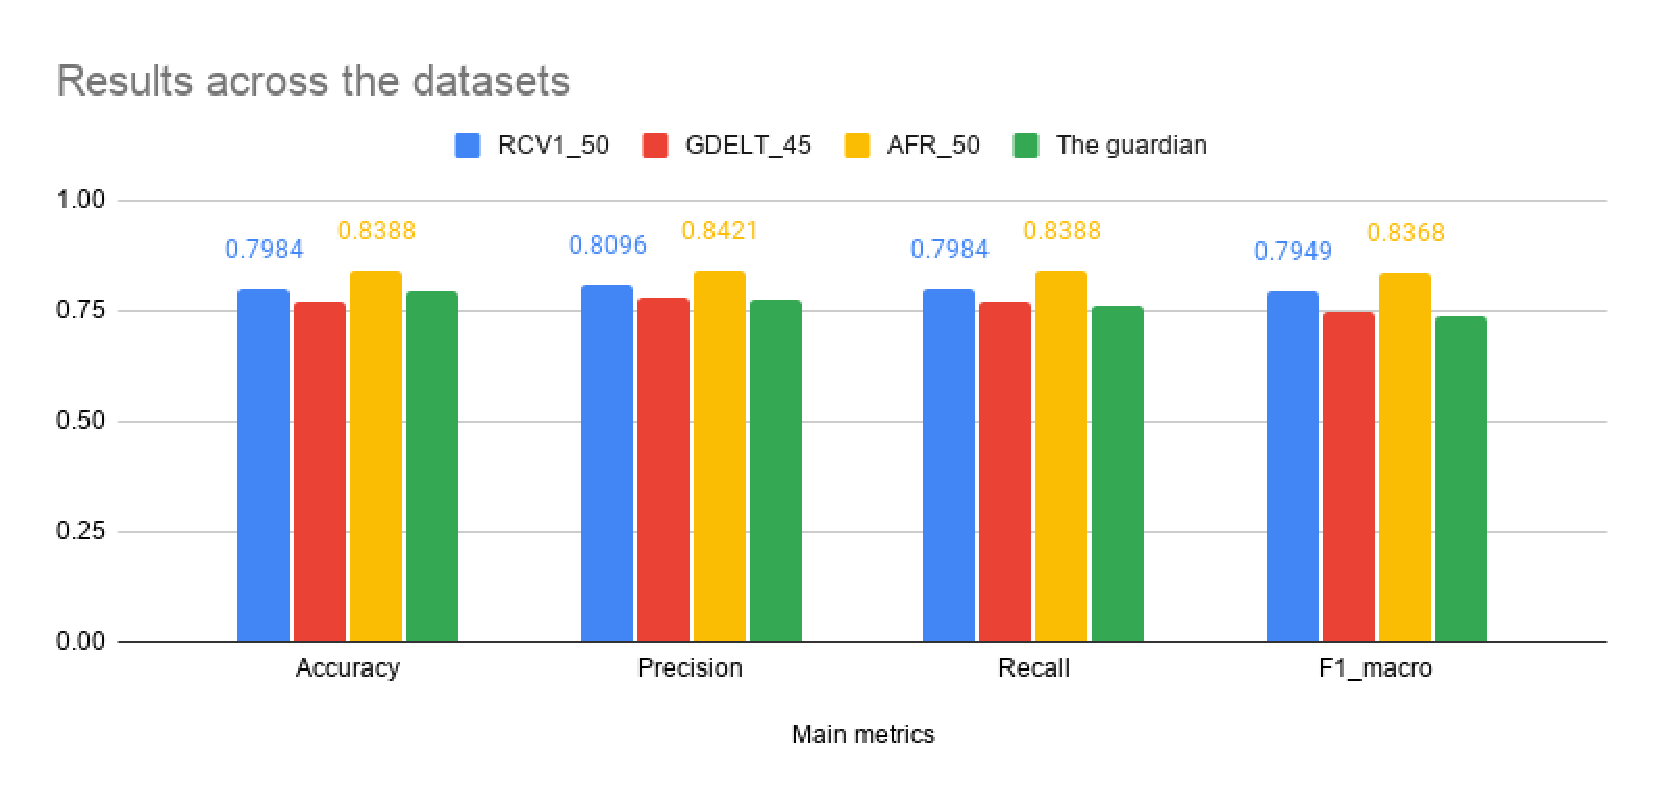
\includegraphics[width=1.0\textwidth, height=1.0\textheight, keepaspectratio]{Results_across_datasets}
	\caption[Best performance across all datasets]{Accuracy, precision, recall and F1 for every dataset showing only the best result achieved for each one.}
	\label{fig:results_across_datasets}
\end{figure}
